%%
%% This is file `sample-sigconf.tex',
%% generated with the docstrip utility.
%%
%% The original source files were:
%%
%% samples.dtx  (with options: `sigconf')
%% 
%% IMPORTANT NOTICE:
%% 
%% For the copyright see the source file.
%% 
%% Any modified versions of this file must be renamed
%% with new filenames distinct from sample-sigconf.tex.
%% 
%% For distribution of the original source see the terms
%% for copying and modification in the file samples.dtx.
%% 
%% This generated file may be distributed as long as the
%% original source files, as listed above, are part of the
%% same distribution. (The sources need not necessarily be
%% in the same archive or directory.)
%%
%%
%% Commands for TeXCount
%TC:macro \cite [option:text,text]
%TC:macro \citep [option:text,text]
%TC:macro \citet [option:text,text]
%TC:envir table 0 1
%TC:envir table* 0 1
%TC:envir tabular [ignore] word
%TC:envir displaymath 0 word
%TC:envir math 0 word
%TC:envir comment 0 0
%%
%%
%% The first command in your LaTeX source must be the \documentclass command.
\documentclass[sigconf]{acmart}

%%
%% \BibTeX command to typeset BibTeX logo in the docs
\AtBeginDocument{%
  \providecommand\BibTeX{{%
    \normalfont B\kern-0.5em{\scshape i\kern-0.25em b}\kern-0.8em\TeX}}}

% %% Rights management information.  This information is sent to you
% %% when you complete the rights form.  These commands have SAMPLE
% %% values in them; it is your responsibility as an author to replace
% %% the commands and values with those provided to you when you
% %% complete the rights form.
% \setcopyright{acmcopyright}
% \copyrightyear{2018}
% \acmYear{2018}
% \acmDOI{10.1145/1122445.1122456}

% %% These commands are for a PROCEEDINGS abstract or paper.
% \acmConference[Woodstock '18]{Woodstock '18: ACM Symposium on Neural
%   Gaze Detection}{June 03--05, 2018}{Woodstock, NY}
% \acmBooktitle{Woodstock '18: ACM Symposium on Neural Gaze Detection,
%   June 03--05, 2018, Woodstock, NY}
% \acmPrice{15.00}
% \acmISBN{978-1-4503-XXXX-X/18/06}


%%
%% Submission ID.
%% Use this when submitting an article to a sponsored event. You'll
%% receive a unique submission ID from the organizers
%% of the event, and this ID should be used as the parameter to this command.
%%\acmSubmissionID{123-A56-BU3}

%%
%% The majority of ACM publications use numbered citations and
%% references.  The command \citestyle{authoryear} switches to the
%% "author year" style.
%%
%% If you are preparing content for an event
%% sponsored by ACM SIGGRAPH, you must use the "author year" style of
%% citations and references.
%% Uncommenting
%% the next command will enable that style.
%%\citestyle{acmauthoryear}

\usepackage{hyperref}
\usepackage{mdframed}
\usepackage{lipsum}
\usepackage{amsmath}
% \usepackage{amssymb}
\usepackage{amsfonts}
\usepackage{ifpdf}
\usepackage{todonotes}
\usepackage{booktabs} % For formal tables
\usepackage{url}
% \usepackage{amssymb}% http://ctan.org/pkg/amssymb
\usepackage{pifont}% http://ctan.org/pkg/pifont
% \usepackage{color}
\usepackage{tcolorbox}
\usepackage{balance}
\usepackage{makecell}
\usepackage{verbatim}
\usepackage{svg}
%\usepackage{cite}
\usepackage{rotating}

\usepackage{stfloats}

\usepackage{bussproofs}
\usepackage{lipsum} % just for the example
\usepackage{mathpartir}
% *** CITATION PACKAGES ***
% *** GRAPHICS RELATED PACKAGES ***
%
% *** MATH PACKAGES ***

% *** SPECIALIZED LIST PACKAGES ***
\usepackage{algorithmic}
\usepackage{listings}
% *** ALIGNMENT PACKAGES ***
\usepackage{array}


% *** SUBFIGURE PACKAGES ***
\usepackage{caption}
%\usepackage{subcaption}
\usepackage{multirow}
\usepackage{float}
\usepackage{mwe}
% *** FLOAT PACKAGES ***
%\usepackage{stfloats}
%\newcommand{\code}[1]{{\fontfamily{cmtt}\fontseries{m}\fontshape{n}\selectfont\smaller{#1}}}
\newcommand{\code}[1]{{\fontfamily{cmtt}\fontseries{m}\fontshape{n}\selectfont\small{#1}}}


\newcommand{\TBD}{{\color{red}(TBD)}}
\newcommand{\haoyu}[1]{{\textcolor{red}{#1}}}


% *** PDF, URL AND HYPERLINK PACKAGES ***
\usepackage{url}
\usepackage{listings}
\lstset{frame=tb,
  language=Python,
  aboveskip=2mm,
  belowskip=1mm,
  showstringspaces=false,
  columns=flexible,
  basicstyle={\small\ttfamily},
  numbers=left,
  numberstyle=\tiny\color{gray},
  keywordstyle=\color{blue},
  commentstyle=\color{dkgreen},
  breaklines=true,
  breakatwhitespace=true,
  tabsize=3,
  xleftmargin=1.5em,
  framextopmargin=0em,
  framexleftmargin=1em
} 

\usepackage{todonotes}
%$\Large\color{green}{\checkmark}$
\newcommand{\cmark}{\ding{51}}%
\newcommand{\xmark}{\ding{55}}%

\usepackage{subfigure}

\usepackage{tikz}
\usetikzlibrary{
  arrows.meta,
  chains,
  matrix,
  positioning,
}
\usepackage{xcolor}
\definecolor{dkgreen}{rgb}{0,0.6,0}

\newcommand*\circled[1]{\tikz[baseline=(char.base)]{
            \node[shape=circle,inner sep=0.8pt] (char) {\textcolor{red}{#1}};}}
            
            
\usepackage[para]{threeparttable}

% local packages
\usepackage{algorithm2e}
\usepackage{xcolor}

%----------------------------------
% custom style commands
%----------------------------------
% variable style command
\newcommand{\xvar}[1]{\textsf{#1}}

% horizontal alignment command
\newcommand{\xvbox}[2]{\makebox[#1][l]{#2}}

%----------------------------------
% set algorithm2e styles
%----------------------------------
% change algorithm font size
\SetAlFnt{\footnotesize}

% change algorithm caption style
\newcommand{\xAlCapSty}[1]{\small\sffamily\bfseries\MakeUppercase{#1}}
\SetAlCapSty{xAlCapSty}

% comment style (algorithms)
\newcommand{\xCommentSty}[1]{\scriptsize\ttfamily\textcolor{blue}{#1}}
\SetCommentSty{xCommentSty}

% change line number style
\newcommand\mynlfont[1]{\scriptsize\sffamily{#1}}
\SetNlSty{mynlfont}{}{} 

 % add the line numbers
\LinesNumbered

% comments right justified
\SetSideCommentRight

% don't print semicolon
\DontPrintSemicolon

% ruled algorithm
\RestyleAlgo{algoruled}

\graphicspath{ {./imgs/} }
%%
%% end of the preamble, start of the body of the document source.
\begin{document}

%%
%% The "title" command has an optional parameter,
%% allowing the author to define a "short title" to be used in page headers.
\title{CG Project Report \\ interactive Texture Based Isosurface Rendering}

%%
%% The "author" command and its associated commands are used to define
%% the authors and their affiliations.
%% Of note is the shared affiliation of the first two authors, and the
%% "authornote" and "authornotemark" commands
%% used to denote shared contribution to the research.
\author{Kaoxin Yao}
\authornote{All two authors contributed equally to this research.}
\affiliation{%
  \institution{Shanghaitech University}
  \city{Shanghai}
  \country{China}
}
\email{yaokx@shanghaitech.edu.cn}

\author{Siyuan Zhang*}
\affiliation{%
  \institution{Shanghaitech University}
  \city{Shanghai}
  \country{China}
}
\email{zhangsy3@shanghaitech.edu.cn}



%%
%% By default, the full list of authors will be used in the page
%% headers. Often, this list is too long, and will overlap
%% other information printed in the page headers. This command allows
%% the author to define a more concise list
%% of authors' names for this purpose.
% \renewcommand{\shortauthors}{Liu Tong Group.}

%%
%% The abstract is a short summary of the work to be presented in the
%% article.
\begin{abstract}

Abstract.

\end{abstract}

%%
%% The code below is generated by the tool at http://dl.acm.org/ccs.cfm.
%% Please copy and paste the code instead of the example below.
%%
\begin{CCSXML}
<ccs2012>
   <concept>
       <concept_id>10010405.10010455.10010460</concept_id>
       <concept_desc>Applied computing~Economics</concept_desc>
       <concept_significance>300</concept_significance>
       </concept>
   <concept>
       <concept_id>10010147.10010178.10010199</concept_id>
       <concept_desc>Computing methodologies~Planning and scheduling</concept_desc>
       <concept_significance>300</concept_significance>
       </concept>
 </ccs2012>
\end{CCSXML}



%%
%% Keywords. The author(s) should pick words that accurately describe
%% the work being presented. Separate the keywords with commas.
\keywords{}

%% A "teaser" image appears between the author and affiliation
%% information and the body of the document, and typically spans the
%% page.


%%
%% This command processes the author and affiliation and title
%% information and builds the first part of the formatted document.
\maketitle

\section{Introduction}

introduction
In this project, we need to render the isosurface by using the volume rendering method. In this task, our team compared two acceleration structures, octree and texture, and finally chose texture acceleration to achieve \textbf{real-time} rendering. By using a simple and convenient UI interface, we were able to adjust the color mapping of the transfer function, change the sampling step, change the viewing angle, and switch between two pre-intergrated tranfer functions.

In the subsequent subheadings of INTRODUCTION, I will describe some of the fundamentals of the content we use.

\subsection{Isosurface}
An isosurface is a three-dimensional analog of an isoline. It is a surface that represents points of a constant val within a volume of space. in other words, it is a level set of a continuous function whose domain is 3D-space.

\begin{figure}
    \centering
    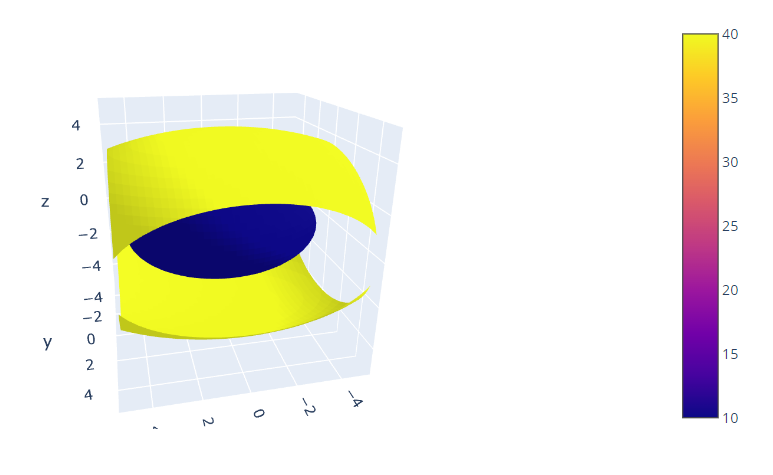
\includegraphics[scale=0.4]{../imgs/isosurface.png}
    \caption{a case of an Iso-surface rendering}
    \label{fig:isocase}
\end{figure}


\subsection{Octree Accelerate Structure}
An octree is a tree-like data structure used to describe a three-dimensional space. Each node of the octree represents a volume element of a cube, and each node has eight child nodes. As a result, we can combine the eight child nodes into a single parent node to complete the tree structure.\cite{Knoll2006InteractiveIR}.
According to the report\cite{SHTUCS1728:online} as shown in \ref{octb}, the Octree-accelerated Isosurface rendering has a very good acceleration ratio, although it does not achieve real-time results.
\begin{figure}
    \centering
    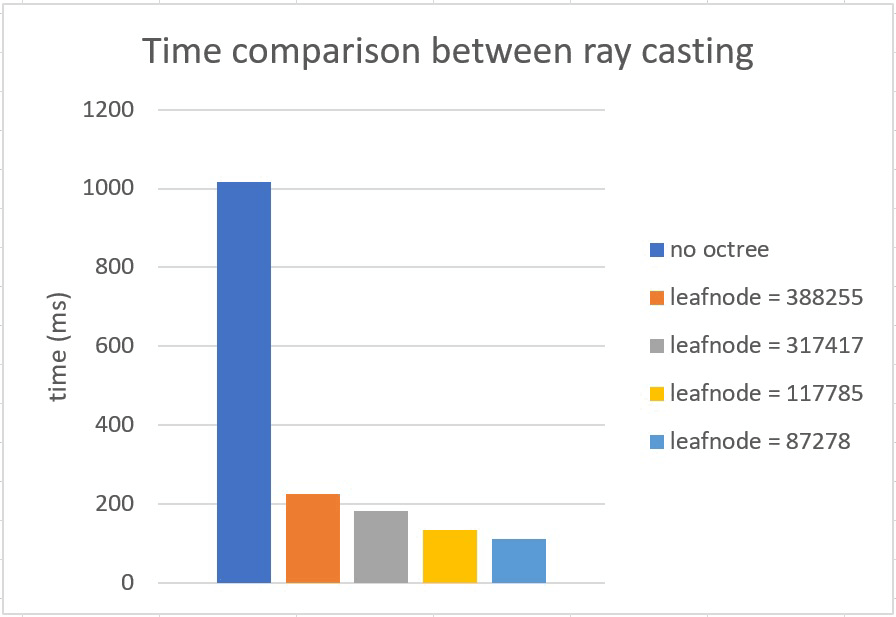
\includegraphics[width=0.4\textwidth]{imgs/octb.png}
    \caption{A Comparison of using Octree or not\cite{SHTUCS1728:online}}
    \label{fig:octb}
\end{figure}
\begin{figure}
    \centering
    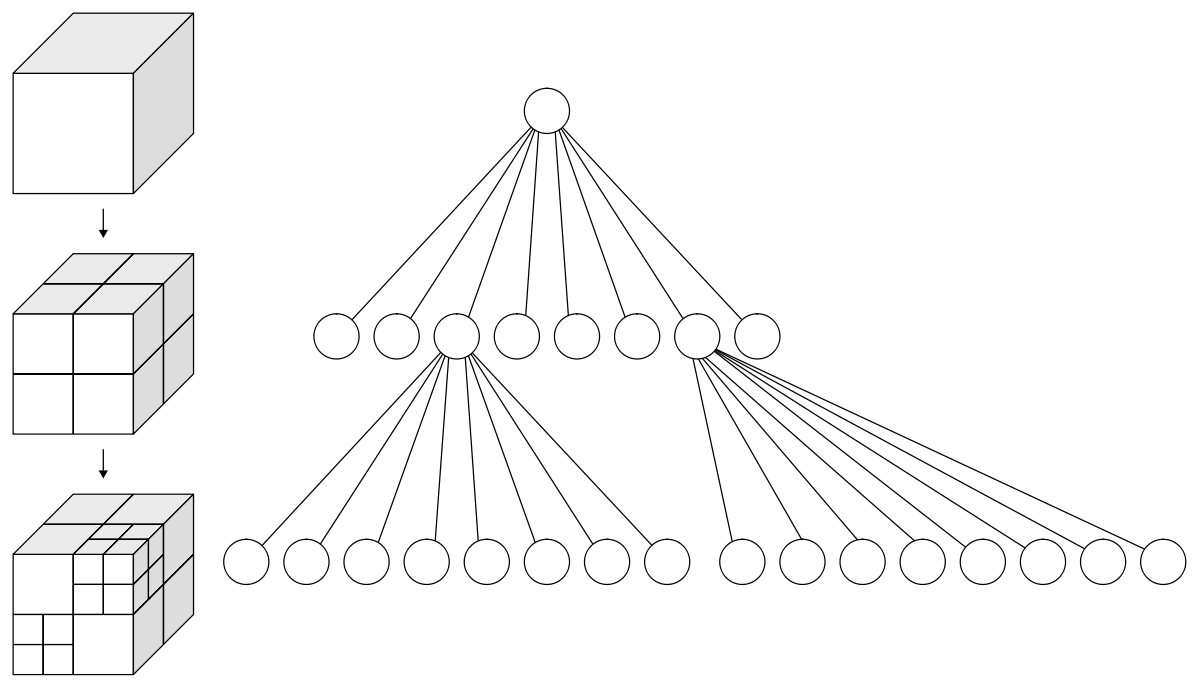
\includegraphics[width=0.4\textwidth]{../imgs/octree.png}
    \caption{Octree Schematic diagram}
    \label{fig:oct1}
\end{figure}

\begin{figure}
    \centering
    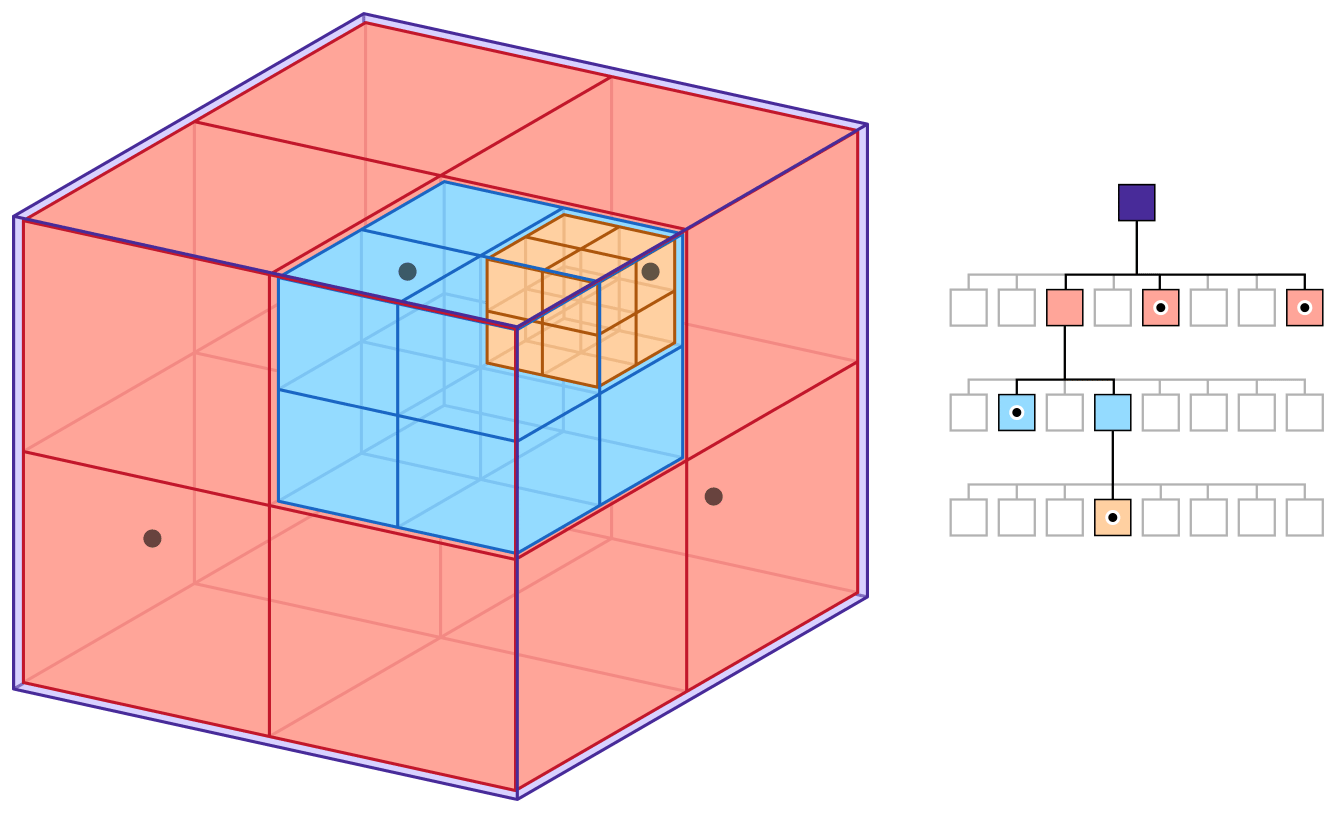
\includegraphics[width=0.4\textwidth]{../imgs/octree2.png}
    \caption{Octree in Volume}
    \label{fig:octreevol}
\end{figure}


\subsection{Pre-integrated transfer function}
The classic transfer function based on interpolation contains two techniques, which are introduced in a popular way, namely post-intergrated transfer function and pre-intergrated transfer function. The former is the same as interpolating across the data's original value and then converting that use the transfer function. The latter is comparable to transforming the original value of data into processed information and then performing interpolation through the processed information for the processed information. In general, the pre-intergrated transfer function will produce a smoother outcome and avoid aliasing.

\subsection{Volume Rendering}
Volume rendering is a set of techniques used to display a 2D projection of a 3D discretely sampled data set, typically a 3D scalar field.A direct volume render requires every sample value to be mapped to opacity and a color. This has already done by our "transfer function" .

The technique of volume ray casting can be derived directly from the rendering equation. A ray is generated for each desired image pixel. Using a simple camera model, the ray starts at the center of projection of the camera  and passes through the image pixel on the imaginary image plane floating in between the camera and the volume to be rendered. Then the ray is sampled at regular or adaptive intervals throughout the volume. The data is interpolated at each sample point, the transfer function applied to form an RGBA sample, the sample is composited onto the accumulated RGBA of the ray, and the process repeated until the ray exits the volume. The RGBA color is converted to an RGB color and deposited in the corresponding image pixel. The process is repeated for every pixel on the screen to form the completed image.

The discrete volume rendering equation and the Schematic diagram are showed below.

\[
C=\sum_{i=1}^{n}C_i\prod_{j=1}^{i-1}(1-A_j)
\]

\[
A=1 - \prod_{j=1}^{i-1}(1-A_j)
\]
\begin{figure}
    \centering
    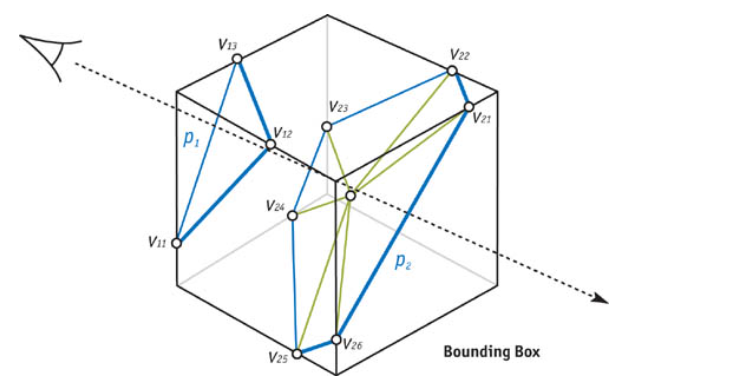
\includegraphics[scale=0.4]{../imgs/volume2.png}
    \caption{Volume Rendering}
\end{figure}


\section{Methodology}

methodology
In the subsequent part of the method, I will describe how we completed the project according to our code logic and the sequence of our experiments

\subsection{Octree Accelerate Structure}
We'll start by reading the data. We can read the information directly because our data is a set of isovalues of size x*y*z. Because the distribution of isovalue is sparse, we can use octree instead of uniformly distributed grids to make the calculation of ray intersections simpler and faster in the following steps. Combining eight grids with the same isovalue into one large grid is more intuitive. In order to prepare for subsequent ray intersections, we process the data into an octree using a recursive approach.

\subsection{Texture Accelerate Structure}
In addition to octree, we can use color preprocessing as texture to further accelerate, because opengl has an excellent texture interpolation function, which can also make each point through gpu interpolation, to achieve the effect of parallelism, and has a better acceleration effect than octree. After comparing the speed, this project chose the texture acceleration method as the core acceleration algorithm, and achieved the effect of real-time acceleration.\cite{httpsdev38:online}

\subsubsection{3D Texture Mapping}
A specific hardware approach has been devised to enable interactive production of view-orthogonal slices. This is an extension of texture-mapping to three-dimensional textures, which is suitably referred to as "3D texturing."
\begin{figure}
    \centering
    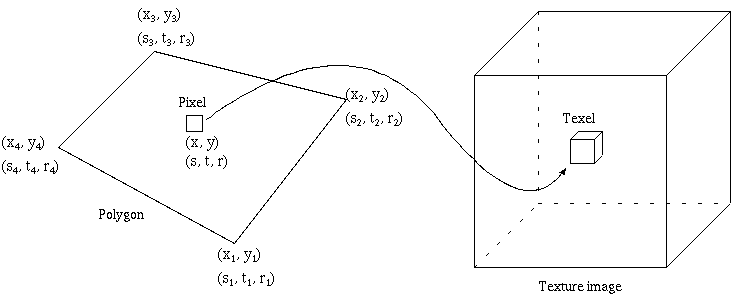
\includegraphics[width=0.4\textwidth]{imgs/TextureMapping3D.png}
    \caption{Calculating color and opacity of a pixel inside a texture-mapped polygon using a 3D texture}
    \label{fig:texture3d}
\end{figure}


The figure above shows how 2D texture-mapping interpolates two additional coordinates (s, t) throughout the interior of a polygon. Three additional coordinates (s, t, r) are interpolated in 3D texture-mapping. These three coordinates are utilized as indices into a three-dimensional image, the 3D texture, to define a pixel's color and opacity, as seen in Figure 6. Tri-linear interpolation is used to recreate texture values.

Because of the GPU's great texture mapping optimization and the fact that we performed the interpolation at the same time as the sample Texture, this calculation is incredibly quick on the GPU.

We primarily employ this strategy as well.

\subsection{Define the transfer function}
Since we already have the structure related to the isovalue, in order to make our results more visualized, we need to define our transfer function, that is, for each cube, we map the known isovalue to the four channels of RGBA. Here, we use a simple UI to manually change the color values corresponding to different isovalues, and map different isovalue layers to the same color. For the A channel, We need to make the transparency selection by associating the value of the point we sampled with the difference between the isovalue and the value of the point, because we only want to render the content of the surface where the isovalue is located. Conversely, the higher the transparency, the smaller the probability that the point is on the surface.

Volumetric data can be treated directly with 3D textures. Rather than constructing a set of two-dimensional slices in a pre-processing step, the volumetric data is downloaded straight into the graphics hardware and used to determine color and opacity values for each pixel covered by a rendered primitive.


\subsection{Different type of Pre-intergated transfer function}
Then we need to perform volume rendering work, we need to obtain the RGBA of each volume, and since we cannot completely sample the known data every time, this results in not only the need to complete the value in the data for the color , the interpolation of value to isovalue and the conversion of transparency also need to complete. For the conversion of value to color, it is divided into two types: pre-intergrated and post-intergrated. In this task, post-intergrated is equivalent to first interpolating the value of the volume (trilinear interpolation), and then passing the interpolated value through The transfer function converts to RGBA, which may cause the color to be not smooth enough, so we prefer to use the pre-intergrated transfer function, which can first obtain RGBA based on known information, and then interpolate to get better and smoother results.

In order to achieve the pre-intergrated function, we initially directly used the establishment of 1D dimensional CDF table as a pre-calculated content, according to our design of the transfer function, we can pre-calculate the RGBA corresponding to each isovalue, in finding the color, we can first find the previous CDF value and the current CDF value by integrating the RGBA on the current isovalue as the color information of the volume.
Therefore, in order to further reduce the error, we also have all isovalue directly projected into a 2D PDF table, directly through the two isovalue values to find more accurate color information.


\subsection{Volume Rendering for Result}
Now that we have a very detailed octree structure with four channels of RGBA, we can use volume rendering to get the final RGB information for each ray. We can directly use the origin and direction of the viewing angle as the light, the light enters the structure, obtains the intersection point with the bounding box, and then obtains a smoother color value according to the preprocessed RGB information and the trilinear interpolation of the cube,the processed alpha information is used as the information for visibility processing, and iteratively passes through volume rendering until the visibility is 1(which means the afterwards things is no longer useful) or all volumes are traversed, and finally the  color result is displayed on the screen.

\subsection{Simple and vivid UI interface}
Considering that the design of isovalue and transfer function is diverse, we use a simple UI interface to help dynamically adjust different isovalues and transfer functions corresponding to different isovalues. We simply do it through the mapping relationship between isovalue and color at this point. In addition to the most important sides, we can also adjust the volume rendering step size, camera position, zoom in and zoom out and other details by pressing the buttons to better show our process of isosurface volume render.




\begin{figure}[]
\center
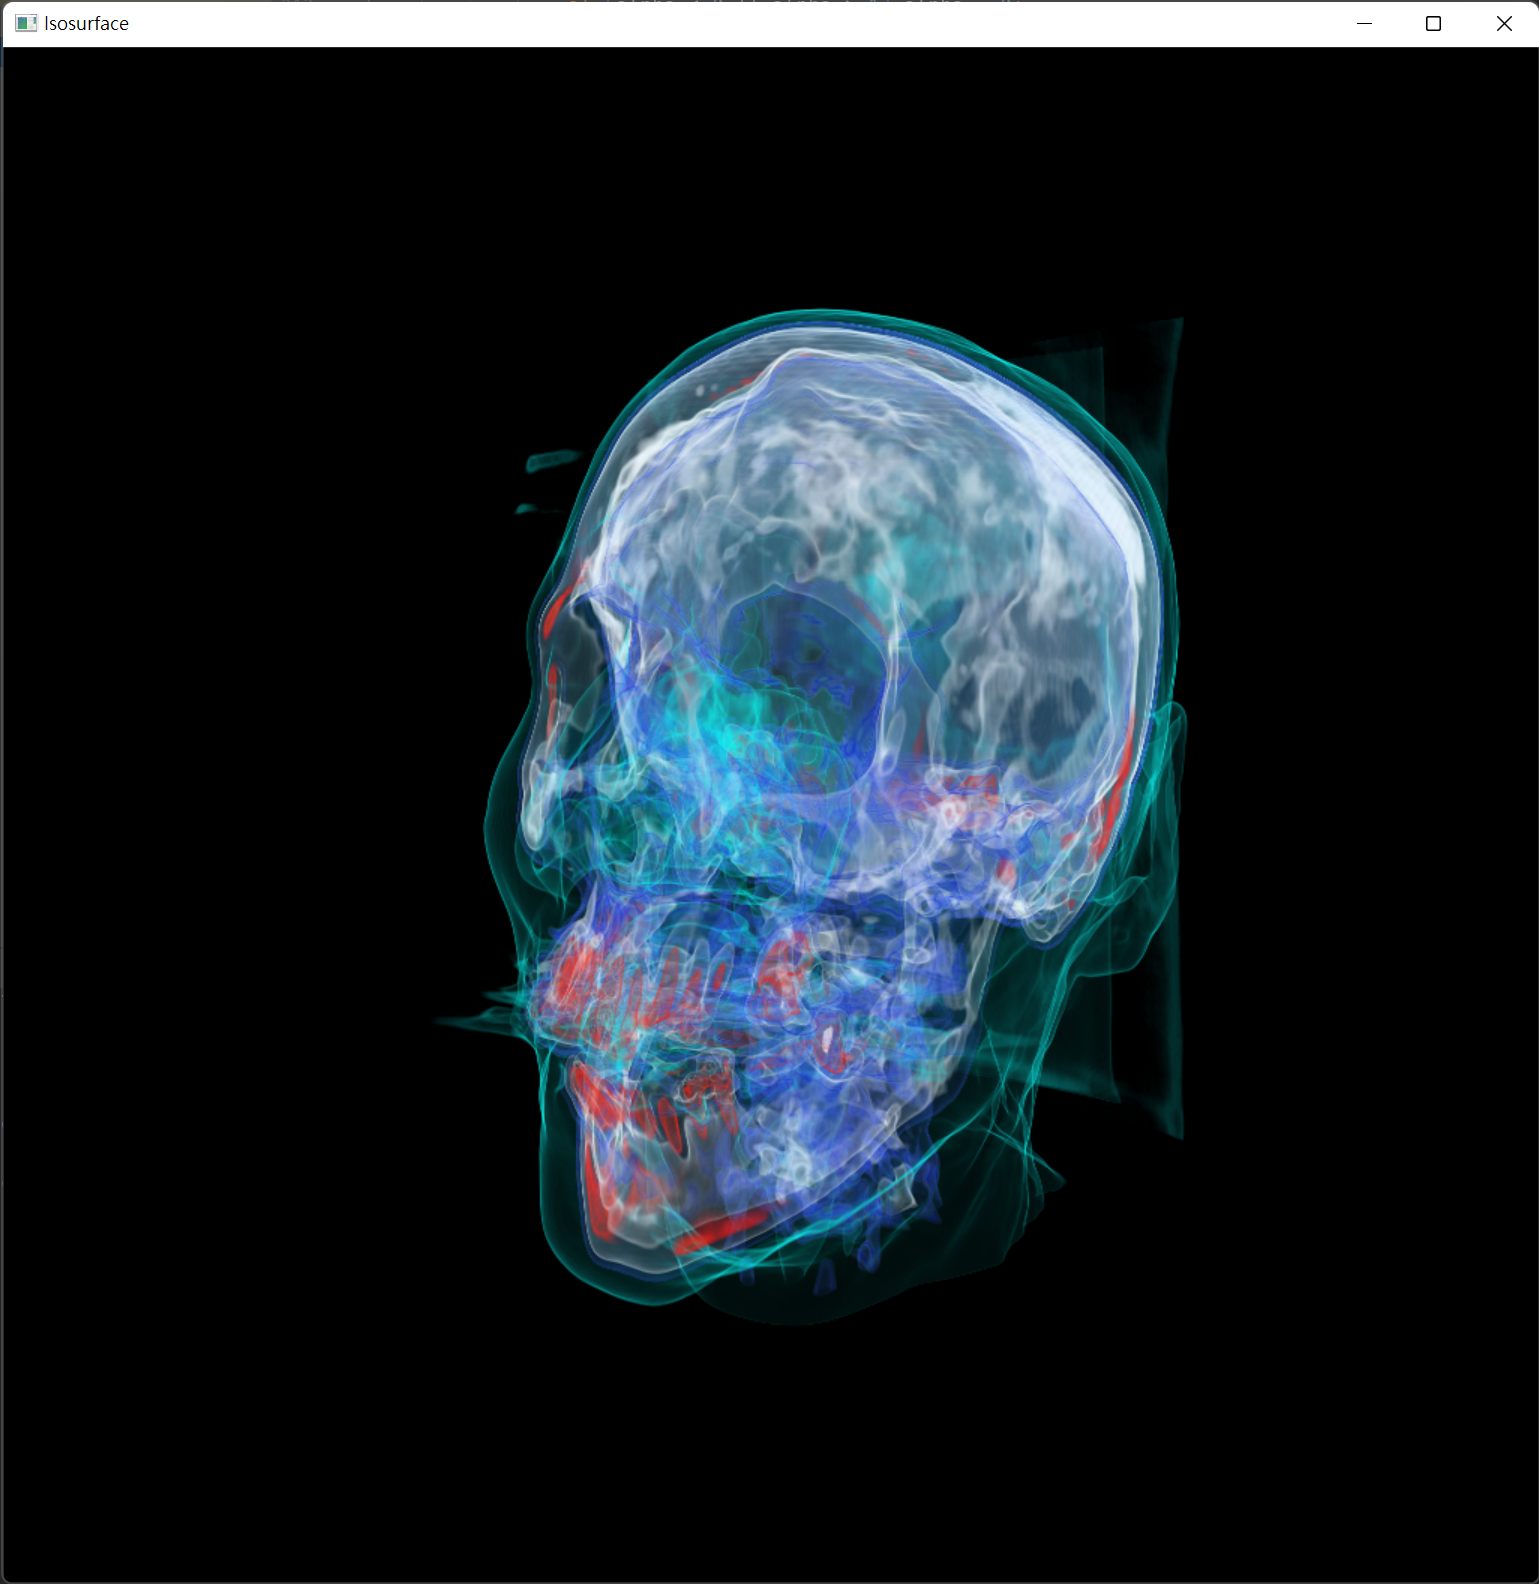
\includegraphics[width=0.4\textwidth]{imgs/cthead.png}
\caption{an Isosurface Rendering Result of a CT Head}
\end{figure}
\begin{figure}[]
\center
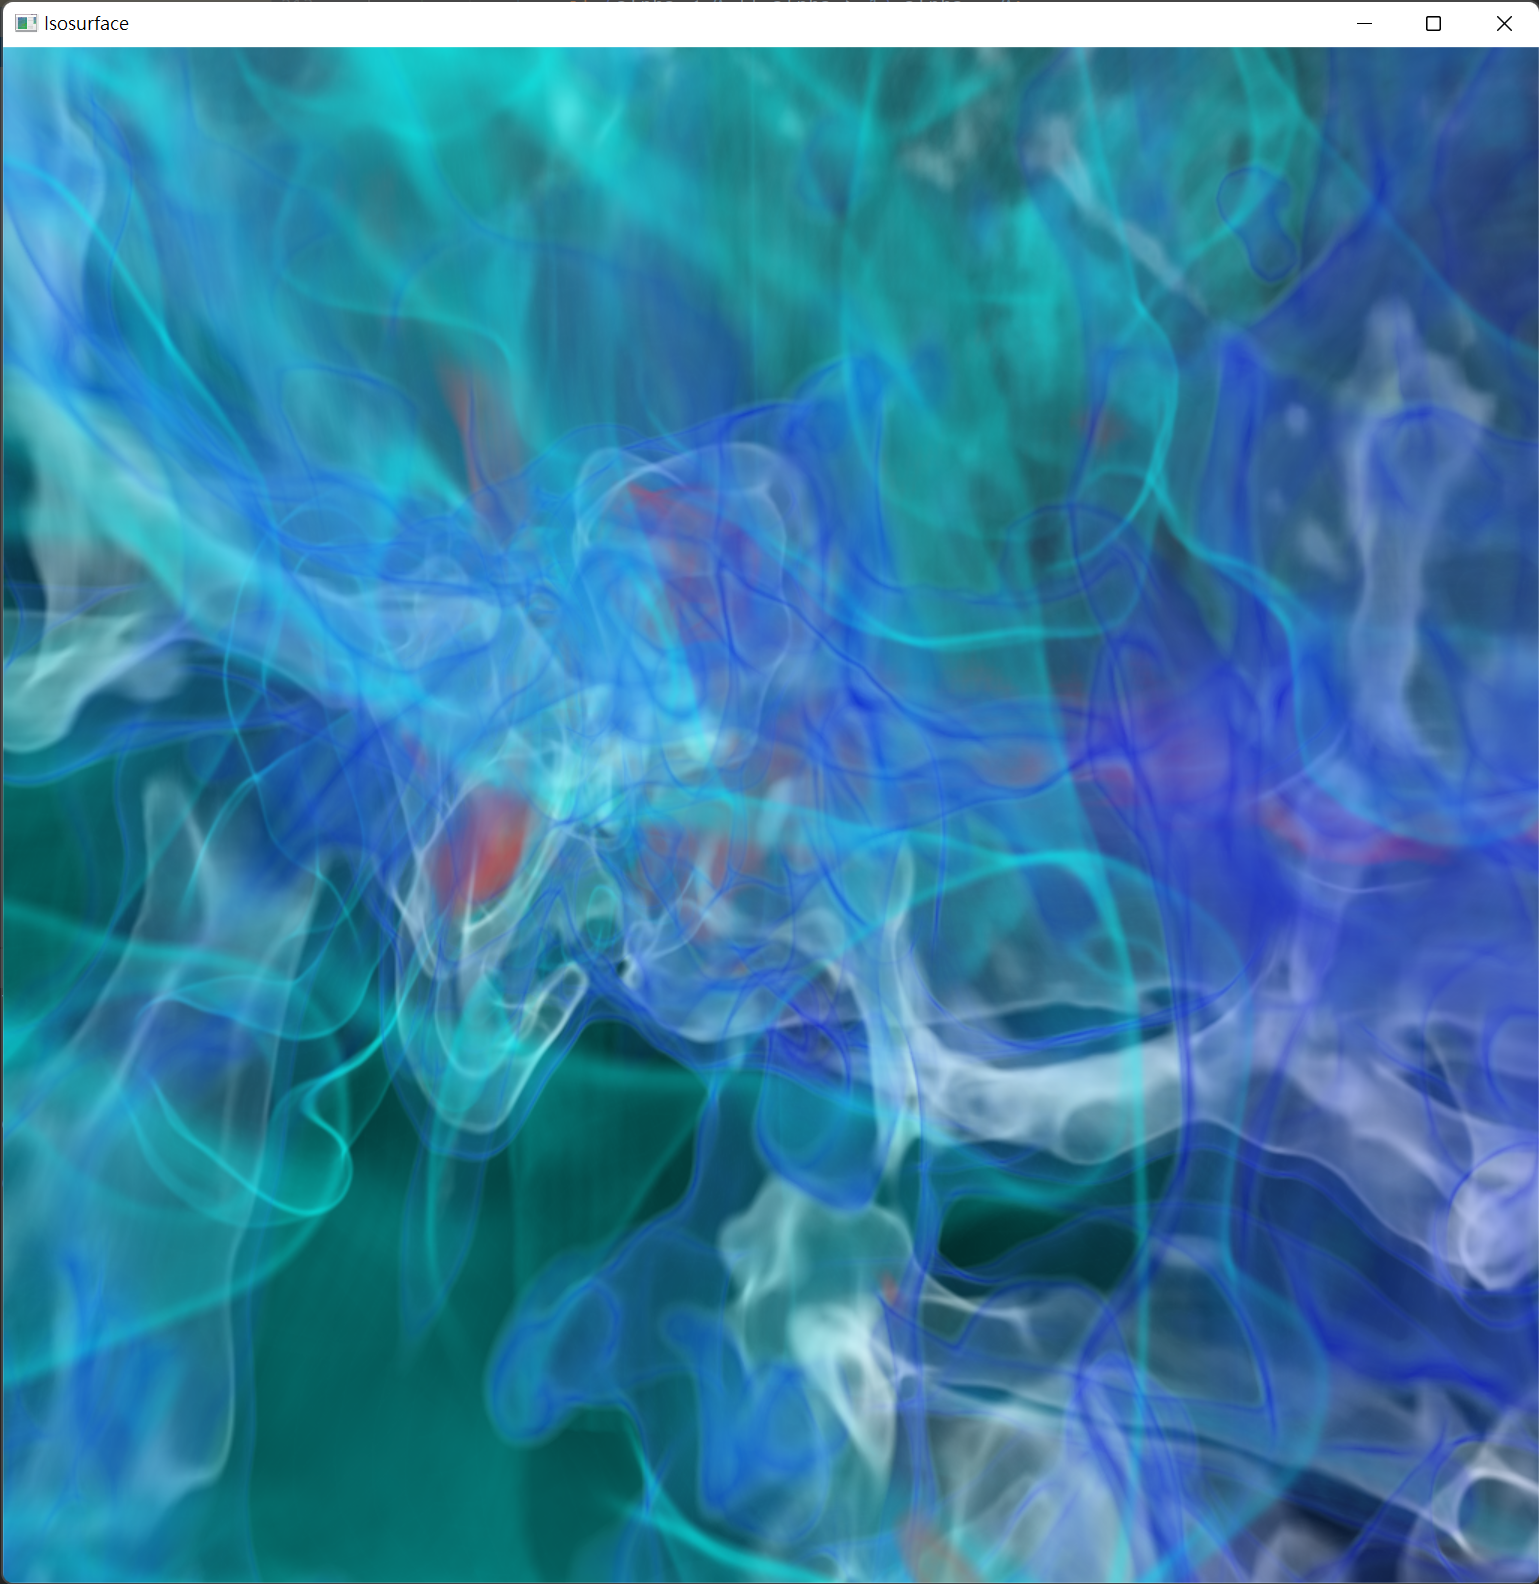
\includegraphics[width=0.4\textwidth]{imgs/close_look.png}
\caption{a Real Close Look of a CT Head}
\end{figure}

\begin{figure}[]
\center
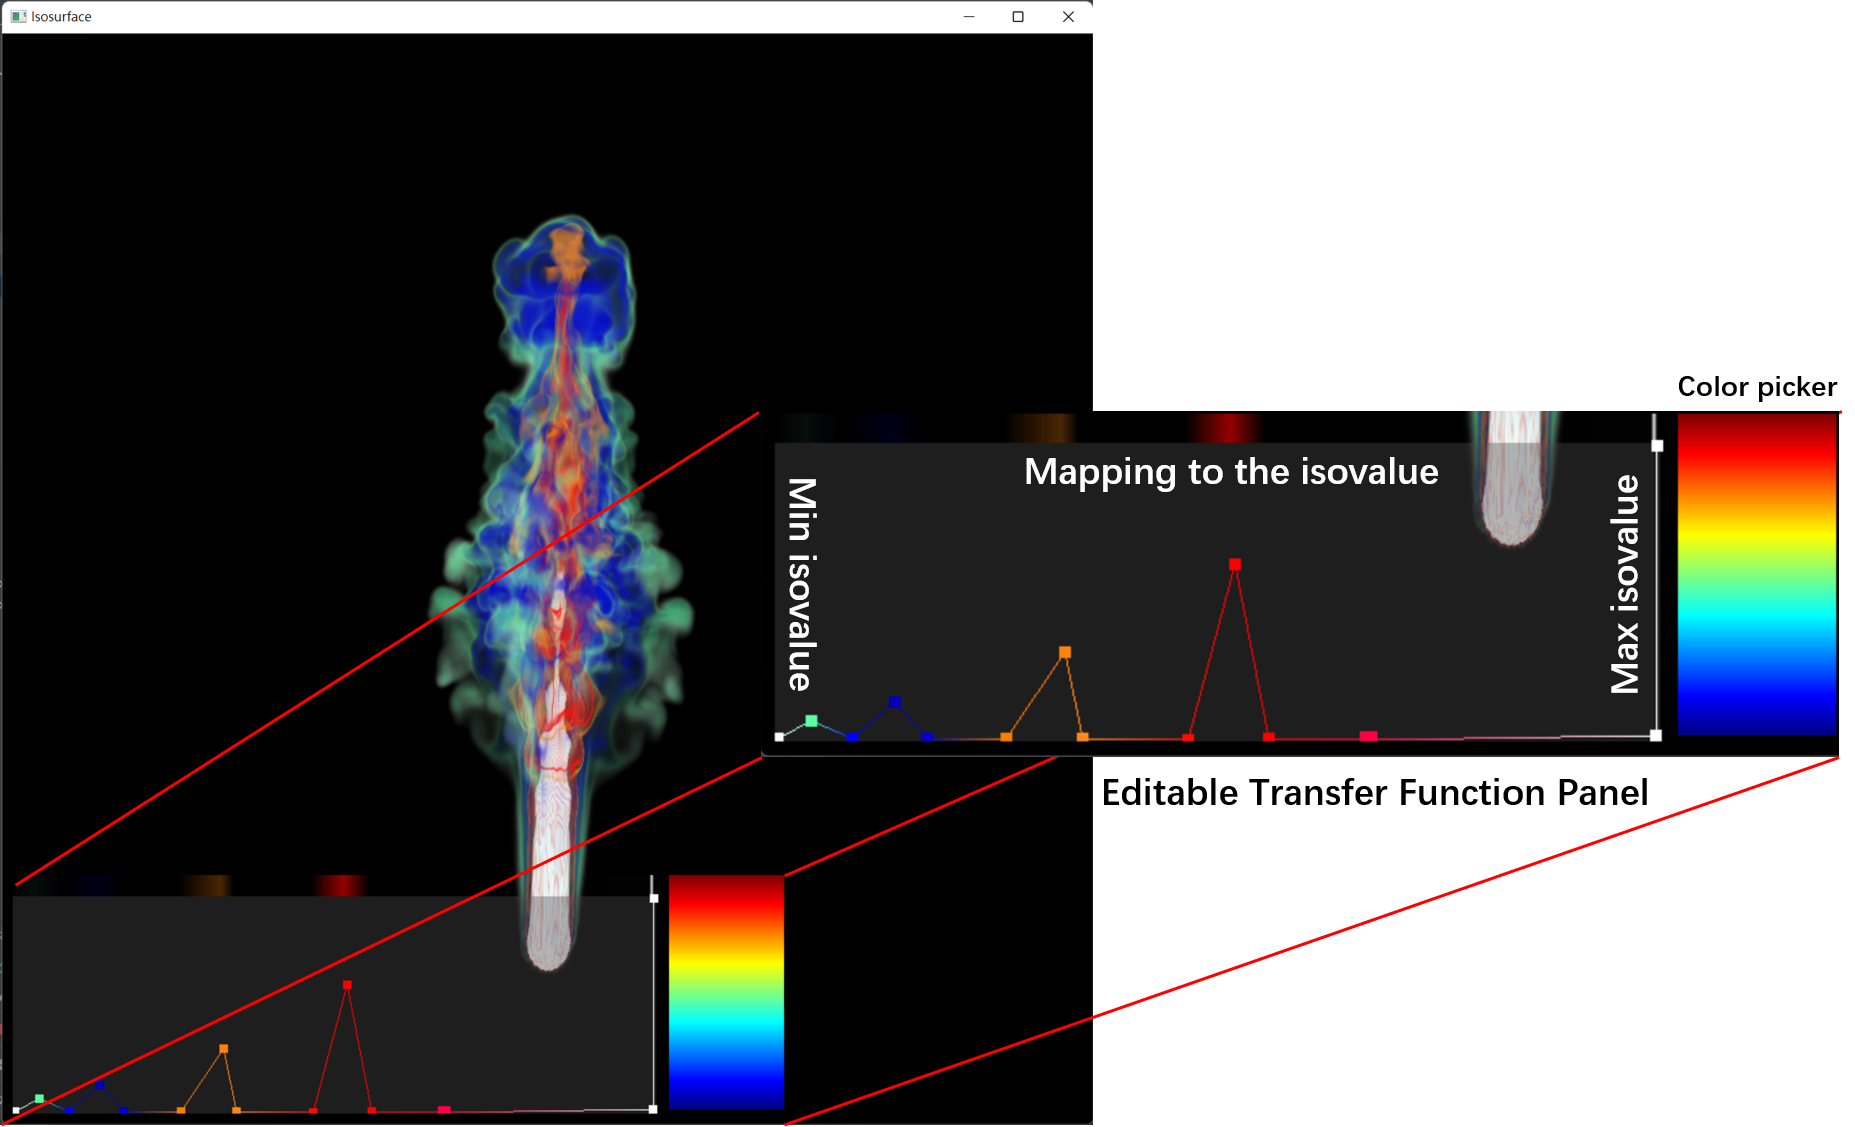
\includegraphics[width=0.4\textwidth]{imgs/panel.png}
\caption{a Simple UI Interface to Change Transfer Function}
\end{figure}

\begin{figure}[]
\center
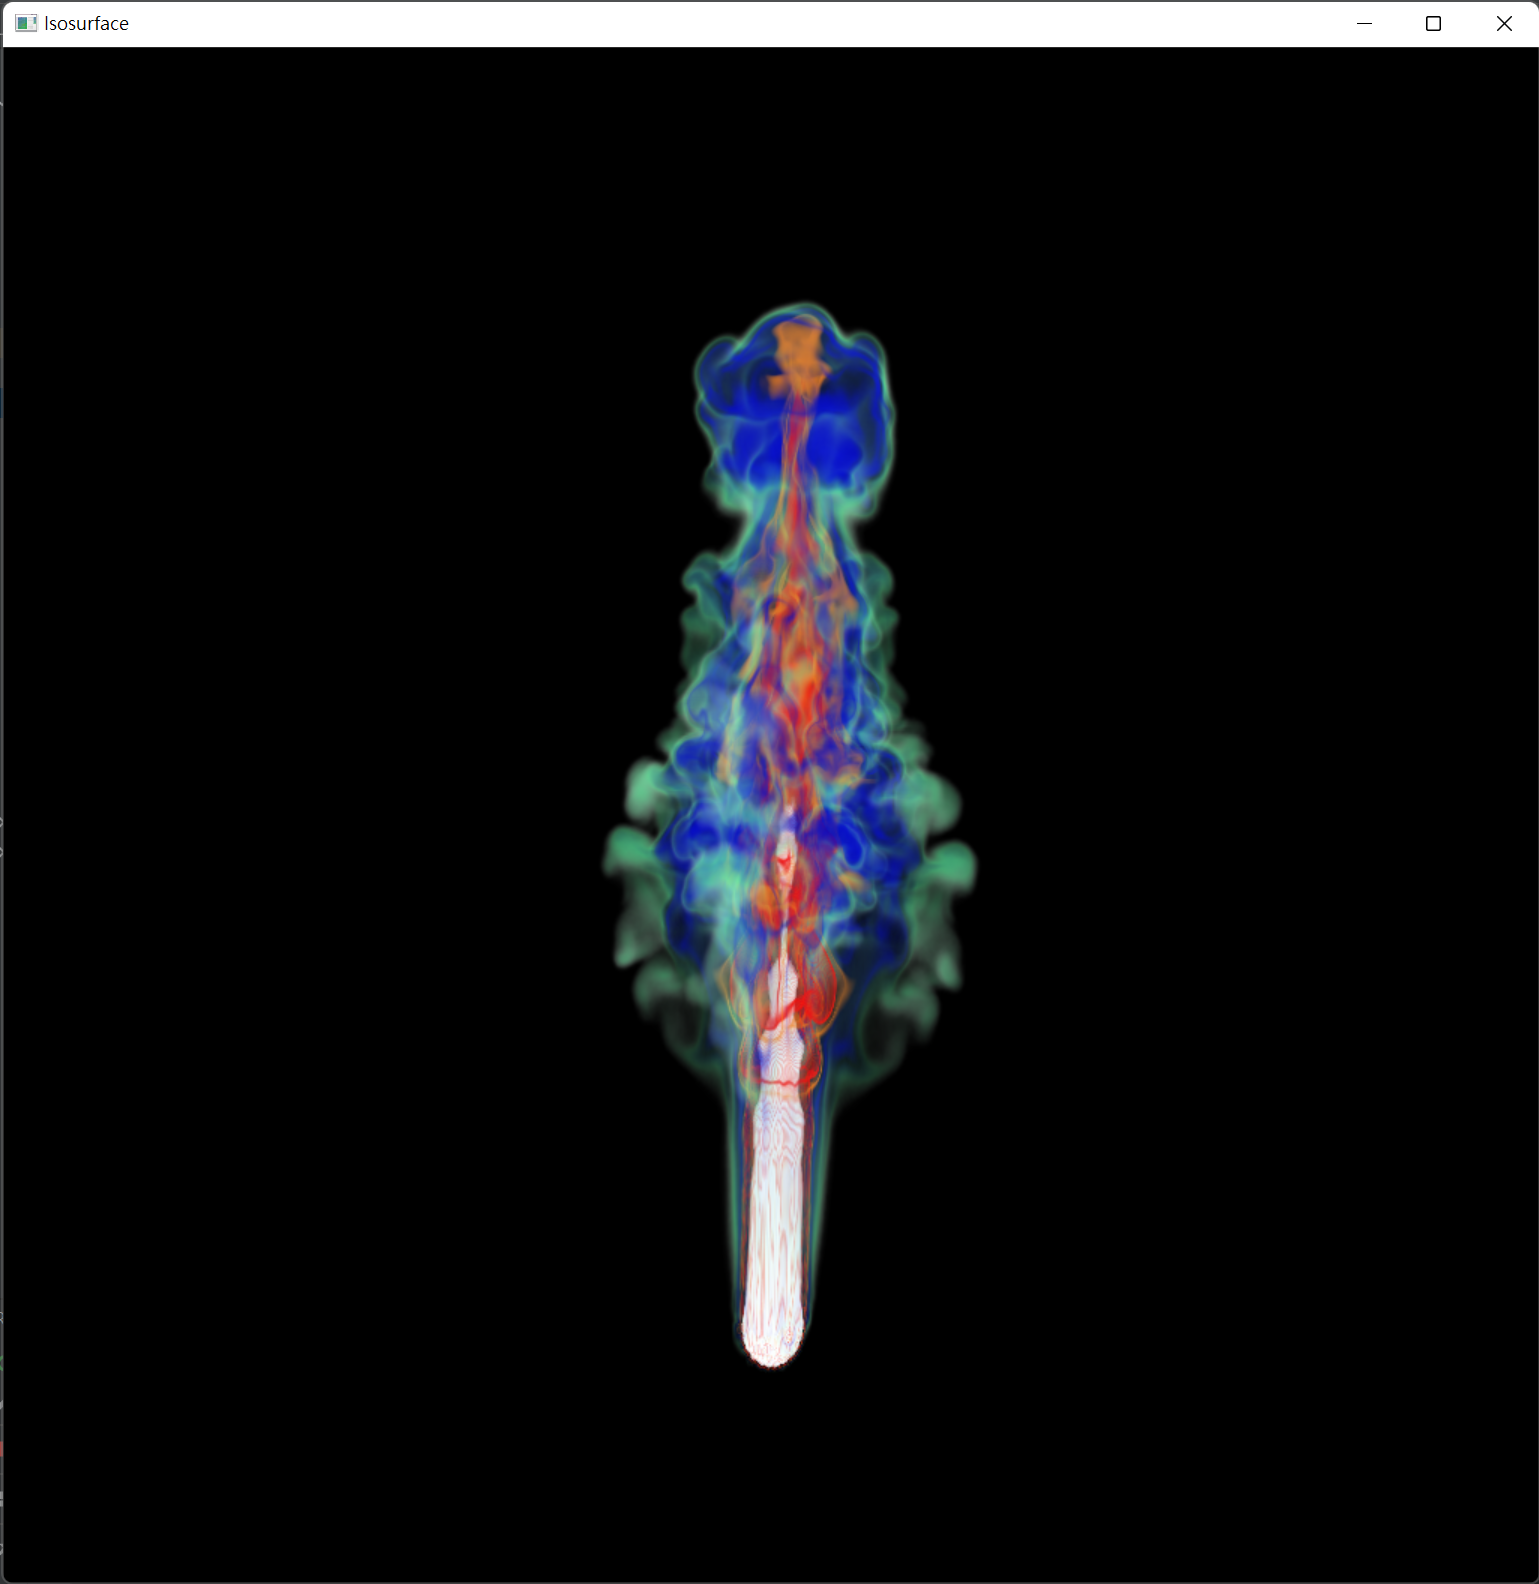
\includegraphics[width=0.4\textwidth]{imgs/flame.png}
\caption{a Isosurface Rendering Result of a Flame}
\end{figure}
\section{code , 3rdlib and reference}

Our code is constructed as figure \ref{code} . 


We use archball\cite{TuvokBas3:online} for control, jet.h for color picker color creation, and other OpenGL-related external libraries. In addition, when writing the code, we referred to the following open source code.\cite{nnagurur86:online}\cite{toolchai50:online}
\begin{figure}
    \centering
    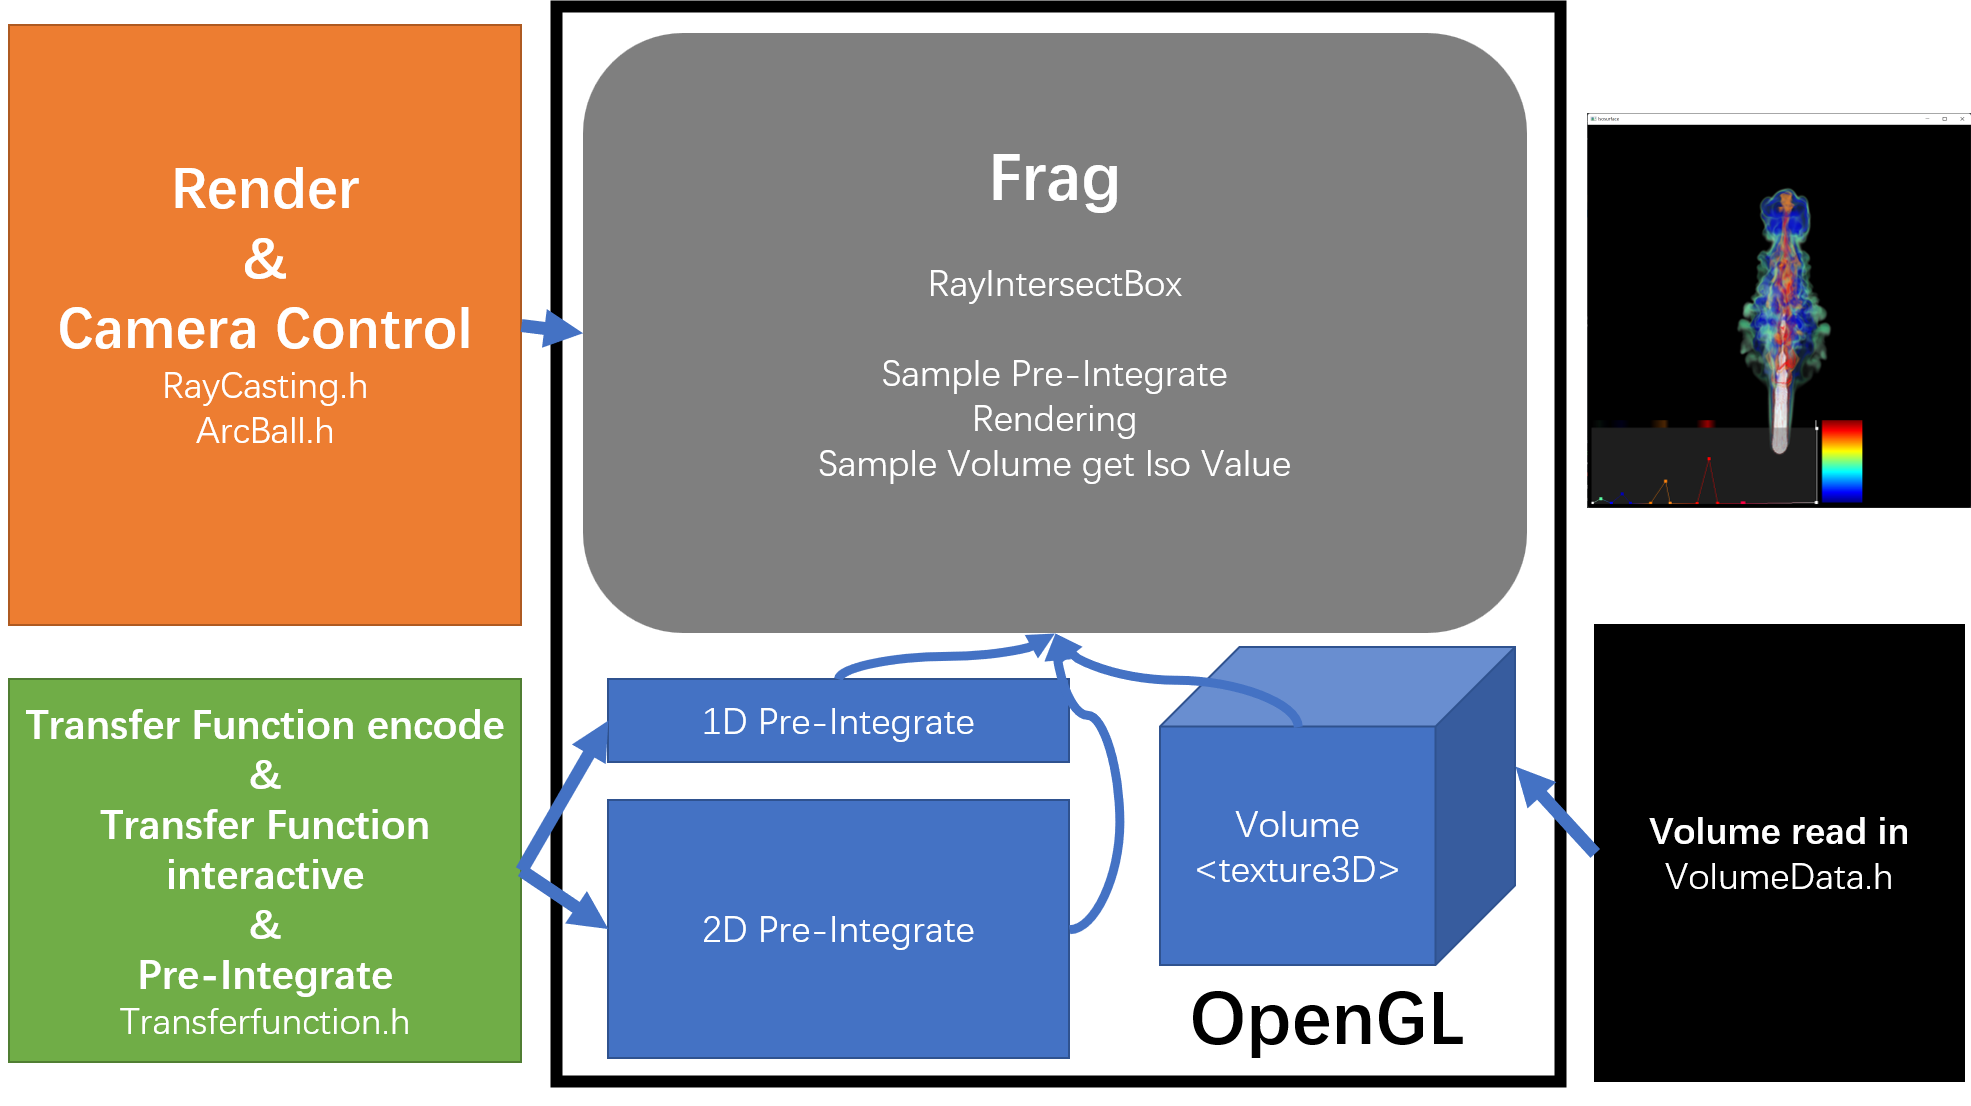
\includegraphics[width=0.5\textwidth]{imgs/code.png}
    \caption{code arch}
    \label{fig:code}
\end{figure}

%%
%% The acknowledgments section is defined using the "acks" environment
%% (and NOT an unnumbered section). This ensures the proper
%% identification of the section in the article metadata, and the
%% consistent spelling of the heading.
% \input{sec/acknowledgments}

%%
%% The next two lines define the bibliography style to be used, and
%% the bibliography file.
\bibliographystyle{ACM-Reference-Format}
\bibliography{reference.bib}

%%
%% If your work has an appendix, this is the place to put it.
% \appendix
% \input{sec/appendix}

\end{document}
\endinput
%%
%% End of file `sample-sigconf.tex'.
